\documentclass[11pt,a4paper]{article}

\usepackage{style2017}
\newcounter{numexo}
\setcellgapes{1pt}

\begin{document}


\begin{NSI}
{Exercice}{Boucles en Python}
\end{NSI}


\addtocounter{numexo}{1}
\subsection*{\Large Exercice \thenumexo }
\begin{enumerate}
\item Donner dans chaque cas les valeurs renvoyées par la boucle \textbf{for}.

\begin{tabular}{p{0.6cm}p{8cm}p{0.6cm}p{8cm}}
\textbf{a)} & \includegraphics[scale=0.8]{img/boucle1.eps} & \textbf{b)} &
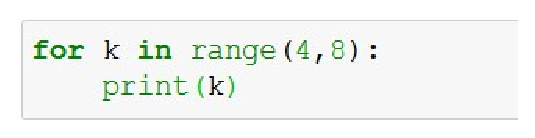
\includegraphics[scale=0.8]{img/boucle2.eps}\\
\textbf{c)} & 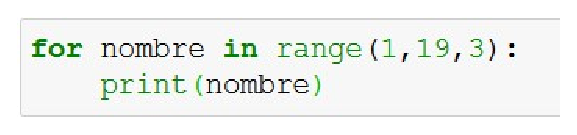
\includegraphics[scale=0.8]{img/boucle3.eps} & \textbf{d)} &
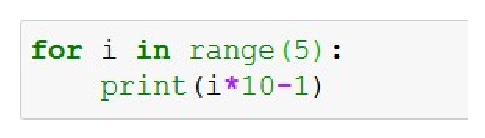
\includegraphics[scale=0.8]{img/boucle4.eps}\\
\end{tabular}\medskip

\item Écrire une boucle for pour obtenir la suite de nombres (sans les virgules) dans chaque cas:
\begin{enumerate}
\item $5, 6, 7, 8, 9$
\item $0, 2, 4, 6, 8, 10, 12, 14, 16, 18$
\item $-1, -2, -3, -4, -5$
\item $4, 9, 16, 25, 36$
\end{enumerate}
\end{enumerate}

\addtocounter{numexo}{1}
\subsection*{\Large Exercice \thenumexo }
Écrire chacune des boucles \textbf{for} de l'exercice 1 avec des boucles \textbf{while} lorsque cela est possible.


\addtocounter{numexo}{1}
\subsection*{\Large Exercice \thenumexo }
\begin{enumerate}
\item Créer une boucle FOR qui affiche 4 fois le message "Bienvenue"
\item Modifier votre programme pour que le message soit affiché autant de fois qu'une valeur saisie avant la boucle.
\item Modifier enfin votre code pour que le message soit numéroté :\\
Bienvenue 1 fois\\
Bienvenue 2 fois\\
etc.
\end{enumerate}

\addtocounter{numexo}{1}
\subsection*{\Large Exercice \thenumexo }
La fonction \textbf{print} affiche un contenu et passe à la ligne. On peut modifier ce comportement en ajoutant un paramètre avec le message.

Par exemple : print("Bienvenue", end="-")

Dans ce cas, à la fin de mot affiché Bienvenue, on a un tiret et on reste sur la même ligne pour l'affichage suivant.

\begin{enumerate}
\item Créer une boucle FOR qui affiche sur une même ligne les nombres de 0 à 9 séparés par un tiret : 0 - 1 -2 -...
\item Modifier votre boucle pour qu'elle affiche les nombres en commençant à 5 : 5 - 6 - 7 - ....
\item Modifier votre boucle qu'elle affiche les nombres progressant de 3 en 3 : 0 - 3 - 6 - ...
\item Modifier votre boucle pour afficher les nombres dans l'ordre décroissant de 9 à 0 : 9 - 8 - 7 - 6 - ...
\end{enumerate}

\addtocounter{numexo}{1}
\subsection*{\Large Exercice \thenumexo }
\begin{enumerate}
\item Écrire un programme qui affiche les nombres de 0 à 99 sur 10 lignes, chaque nombre étant séparé par un tiret.
\item Proposer une seconde version afin qu'il n'y ait pas de tiret à la fin de chaque ligne.
\end{enumerate}

\newpage
\addtocounter{numexo}{1}
\subsection*{\Large Exercice \thenumexo }
\begin{enumerate}
\item On souhaite réaliser le motif en "X" ci-dessous. Il est composé de 10 lignes et 10 colonnes.
\begin{center}
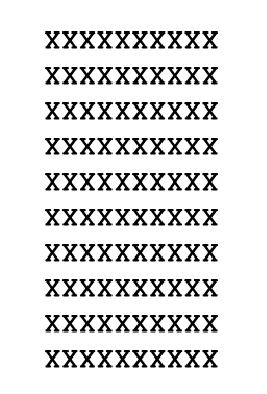
\includegraphics[scale=0.5]{img/carreX.eps}
\end{center}
\begin{enumerate}
\item Créer une première boucle qui permet de créer une première ligne. Pour afficher du texte sur une même ligne, il faut ajouter le paramètre \textbf{end} à la fonction \textbf{print} : print(message, end="").
\item Créer une boucle qui va répéter 10 fois la boucle précédente. On dit que ce sont des boucles imbriquées.
\end{enumerate}
\item Modifier votre code pour que le nombre de lignes et colones soit saisi par l'utilisateur.
\item Réaliser les motifs suivants de 10 lignes et 10 colonnes:

\begin{minipage}{6cm}
\textbf{a)}
\begin{center}
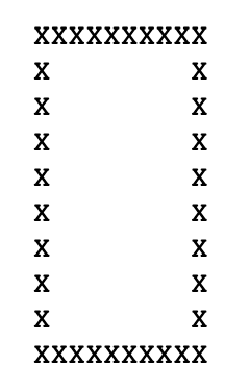
\includegraphics[scale=0.5]{img/carreX2.eps}
\end{center}
\end{minipage}
\begin{minipage}{6cm}
\textbf{b)}
\begin{center}
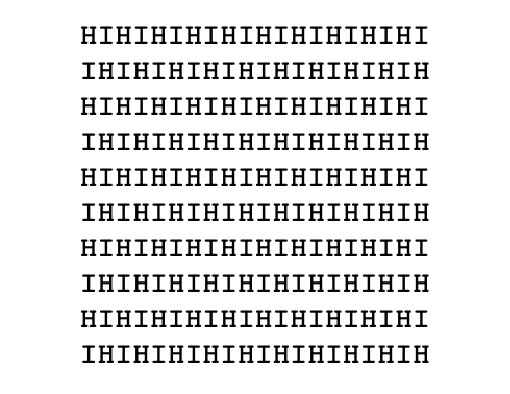
\includegraphics[scale=0.5]{img/carreX4.eps}
\end{center}
\end{minipage}
\begin{minipage}{6cm}
\textbf{c)}
\begin{center}
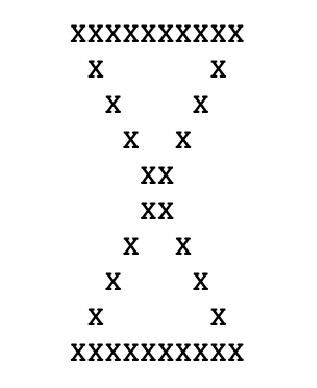
\includegraphics[scale=0.5]{img/carreX6.eps}
\end{center}
\end{minipage}
\end{enumerate}

\addtocounter{numexo}{1}
\subsection*{\Large Exercice \thenumexo }
\begin{enumerate}
\item Écrire un premier programme qui calcule et affiche $1 + 2 + 3 + \ldots + 100$.
\item Écrire un second programme qui calcule et affiche $1 \times 2 \times \ldots \times 100$.
\item Modifier les deux programmes précédents pour calculer et afficher les résultats jusqu'à un nombre $N$ saisi par l'utilisateur.
\end{enumerate}

\addtocounter{numexo}{1}
\subsection*{\Large Exercice \thenumexo }
Les programmes seront appliqués sur la chaine de caractères suivante :
\begin{center}
Le langage python a été créé par Guido Van Rossum.
\end{center}
\begin{enumerate}
\item Écrire un programme qui affiche les voyelles contenues dans la chaine de caractères.
\item Écrire un programme qui affiche la chaine de caractères en lettres capitales.
\item Écrire un programme qui affiche la chaine de caractères écrite à l'envers (lettre par lettre).
\end{enumerate}

\addtocounter{numexo}{1}
\subsection*{\Large Exercice \thenumexo }
\begin{enumerate}
\item Saisir dans l'interpréteur la fonction "bin(9)". Quel est le résultat affiché ?
\item L'objectif est de créer une boucle WHILE qui donne l'écriture binaire d'un nombre entier positif en utilisant les divisions successives.
\begin{enumerate}
\item On utilisera les variables \textbf{n} pour le nombre entier positif, \textbf{b} pour l'écriture binaire obtenue qui sera de type "string" et \textbf{r} pour les restes des divisions entières.   
\item On calculera les divisions en mémorisant le reste dans une variable \textbf{r} et le nouveau quotient dans n.    
\item Le nombre \textbf{n} est divisé par 2 jusquà devenir nul. On fait les calculs tant que \textbf{n} est différent de 0.    
\item On construit le nombre binaire \textbf{b} comme chaine de caractères constituée des restes.
\end{enumerate}
\item On pourra faire une vérification avec la fonction \textbf{int(chaine,base)}.
\end{enumerate}

\end{document}

